\documentclass[serif, 9pt, aspectratio=32]{beamer} 
\usetheme{Darmstadt}

\usepackage{appendixnumberbeamer}
\usepackage{booktabs}
\usepackage[scale=2]{ccicons}
\usepackage{pgfplots}
\usepgfplotslibrary{dateplot}
\usepackage{xspace}
\usepackage{tikz}
\usepackage{hyperref}
\usepackage{xcolor}
\usetikzlibrary{shapes, arrows}
\newcommand{\themename}{\textbf{\textsc{metropolis}}\xspace}

\title{City Location Choice and Houehold Productivity}
\date{\today}
\author{Tan Sein Jone}
\institute{University of British Columbia}

\pgfplotsset{compat=1.18}
\setbeamertemplate{footline}[frame number]

\begin{document}

\maketitle

\begin{frame}{Table of contents}
    \setbeamertemplate{section in toc}[sections numbered]
    \tableofcontents[hideallsubsections]
\end{frame}

\section{Cities}

\begin{frame}
    \frametitle{Table of Contents}
    \setbeamertemplate{section in toc}[sections numbered]
    \tableofcontents[currentsection]
\end{frame}

\begin{frame}
    \centering
    \frametitle{Agglomoration}
    \begin{itemize}
        \setlength{\itemsep}{3em}
        \item According to the world bank, 56\% of the world's population live in cities.
              \begin{itemize}
                  \setlength{\itemsep}{1em}
                  \item This is expected to increase to 70\% by 2050.
              \end{itemize}
        \item People choose to live in cities in spite of problems such as congestion and high rents.
        \item This is because of the benifits cities offer.
              \begin{itemize}
                  \setlength{\itemsep}{1em}
                  \item Households, better work oppotunities and better amenities.
                  \item Businesses, better access to services and a larger market.
              \end{itemize}
    \end{itemize}
\end{frame}

\begin{frame}
    \centering
    \frametitle{Trivial Solution}
    \begin{itemize}
        \setlength{\itemsep}{3em}
        \item If cities are identical and size determines the magnitude of agglomoration benifits, then all households would choose to live in the same city.
        \item Cities are obviously not homogenous.
              \begin{itemize}
                  \item Toronto is not the same as Vancouver.
              \end{itemize}
        \item Why do people choose to live in the cities they do?
    \end{itemize}
\end{frame}

\begin{frame}
    \centering
    \frametitle{Research Question}
    \begin{itemize}
        \setlength{\itemsep}{3em}
        \item What will happen to city populations when there's a shock to the economy?
              \begin{itemize}
                  \item What will the migration patterns look like?
              \end{itemize}
        \item How substitutable are cities?
              \begin{itemize}
                  \item How do households choose between cities?
              \end{itemize}
        \item With city heterogeneity, can we break the independence of irrelevant alternatives (IIA) assumption in spacial econ?
              \begin{itemize}
                  \item Cities are not directly substitutable for each other.
              \end{itemize}
    \end{itemize}
\end{frame}

\section{Background}

\begin{frame}
    \frametitle{Table of Contents}
    \setbeamertemplate{section in toc}[sections numbered]
    \tableofcontents[currentsection]
\end{frame}

\begin{frame}
    \centering
    \frametitle{Eaton and Kortum (2002)}
    \begin{itemize}
        \setlength{\itemsep}{3em}
        \item Ricardian Model of Trade
              \begin{itemize}
                  \item Countries should perfectly specialize in the production of goods they have a comparative advantage in.
              \end{itemize}
        \item Probabalistic draws of Productivity
              \begin{itemize}
                  \item Draw from a Frechet distribution.
                  \item For a variety of goods, what is the probability you can produce below a certain price?
              \end{itemize}
        \item Result
              \begin{itemize}
                  \item Non zero production of all goods in all countries.
              \end{itemize}
    \end{itemize}
\end{frame}

\begin{frame}
    \centering
    \frametitle{Redding (2016)}
    \begin{itemize}
        \setlength{\itemsep}{3em}
        \item Quatitative Spacial Model
        \item Take EK and applied to to an urban/spacial setting.
        \item Wages are determined by productivities.
        \item Wages and amenities determine location choice shares.
    \end{itemize}
\end{frame}

\begin{frame}
    \centering
    \frametitle{Lind and Ramondo (2023)}
    \begin{itemize}
        \setlength{\itemsep}{3em}
        \item Trade with Correlation
        \item Preferences
              \begin{itemize}
                  \setlength{\itemsep}{1em}
                  \item EK has CES preferencces where goods are perfectly substitutable.
                  \item Lind and Ramondo proposed a cross nested CES structure in order to break IIA.
                  \item A Lamborghini is not the same as a Toyota.
              \end{itemize}
        \item Better suited substitution patterns in trade.
    \end{itemize}
\end{frame}

\begin{frame}
    \centering
    \frametitle{This Paper}
    \begin{itemize}
        \setlength{\itemsep}{3em}
        \item Apply this new framework that allows for correlation to Redding's QSM.
        \item QSM currently loads city heterogeneity entirely onto amenities.
        \item This paper will attempt to explain some of that variation.
    \end{itemize}
\end{frame}

\section{Model}

\begin{frame}
    \frametitle{Table of Contents}
    \setbeamertemplate{section in toc}[sections numbered]
    \tableofcontents[currentsection]
\end{frame}

\begin{frame}
    \centering
    \frametitle{Setup}
    \begin{itemize}
        \setlength{\itemsep}{3em}
        \item $N$ cities indexed by $c$.
        \item $K$ occupations indexed by $k$.
        \item A continuim of household types $\nu \in [0,1]$.
    \end{itemize}
\end{frame}

\begin{frame}
    \centering
    \frametitle{Setup}
    \begin{itemize}
        \setlength{\itemsep}{3em}
        \item Output is entirely determined by productivity.
        \item Wages are determined by productivity and a city specific price index.
              \begin{itemize}
                  \item The price index will be set to 1 in the baseline model.
              \end{itemize}
        \item Utility is entirely determined by wages.
              \begin{itemize}
                  \item A housheold maximizes utility by choosing the city that maximizes their wage.
              \end{itemize}
    \end{itemize}
\end{frame}

\begin{frame}
    \centering
    \frametitle{Productivity}
    \begin{itemize}
        \setlength{\itemsep}{2em}
        \item Every household in every city occupation pair draws a productivity from this Frechet distribution.
              \vspace{2em}
              \begin{equation}
                  \label{specific_Frechet}
                  \begin{aligned}
                      P[Z_{ck} < z] = exp[-(T_{ck}^{\star} z^{-\theta})^{\frac{1}{1 - \rho_k}}]
                  \end{aligned}
              \end{equation}
    \end{itemize}
    \vspace{3em}
    \begin{itemize}
        \item $T_{ck}^{\star}$ is the city occupation specific productivity scale parameter.
              \begin{itemize}
                  \item This represents a city's absolute advantage in that occupation.
              \end{itemize}
        \item $\theta$ is the Frechet shape parameter.
        \item $\rho_k$ is the occupation correlation parameter.
    \end{itemize}
\end{frame}

\begin{frame}
    \centering
    \frametitle{Correlation Function}
    \begin{itemize}
        \setlength{\itemsep}{2em}
        \item These productivities have a correlation structure.
              \begin{equation}
                  \label{correlation}
                  \begin{aligned}
                      G (Z_1^{-\theta}, \dots, Z_N^{-\theta})= \sum_{k}^{} [\sum_{c}^{N} (T_{ck}^{\star} Z_c^{-\theta})^{\frac{1}{1 - \rho_k}}]^{1 - \rho_k}
                  \end{aligned}
              \end{equation}
    \end{itemize}
    \vspace{2em}
    \begin{itemize}
        \item Cities have correlated draws based on occupations.
        \item $T_{ck}^{\star}$ is what we get when we intergrate over all household types.
    \end{itemize}
\end{frame}

\begin{frame}
    \centering
    \frametitle{Choice Shares}
    \begin{equation}
        \label{choice_shares}
        \begin{aligned}
            \pi_c = \frac{Z_c^{-\theta} G_c(Z_1^{-\theta}, \dots, Z_N^{-\theta})}{G(Z_1^{-\theta}, \dots, Z_N^{-\theta})}
        \end{aligned}
    \end{equation}
    \vspace{2em}
    \begin{equation}
        \label{choice_shares_complete}
        \begin{aligned}
            \pi_c = \frac{T_c^{\star} Z_c^{-\theta}}{\sum_{c}^{N} T_c^{\star} Z_c^{-\theta}}
        \end{aligned}
    \end{equation}
    \vspace{2em}
    \begin{itemize}
        \setlength{\itemsep}{2em}
        \item Choice shares are dependent on productivity shares and city specifc shifters.
    \end{itemize}
\end{frame}

\section{Preliminary Results}

\begin{frame}
    \frametitle{Table of Contents}
    \setbeamertemplate{section in toc}[sections numbered]
    \tableofcontents[currentsection]
\end{frame}

\begin{frame}
    \centering
    \frametitle{Setup}
    \begin{itemize}
        \setlength{\itemsep}{3em}
        \item 3 cities
              \begin{itemize}
                  \setlength{\itemsep}{1em}
                  \item Chicago, Detriot and New York.
                  \item Chicago and Detriot specialise in trades.
                  \item New York specialises in services.
              \end{itemize}
    \end{itemize}
\end{frame}

\begin{frame}
    \centering
    \frametitle{Simulation Results}
    \begin{figure}[h]
        \begin{minipage}{0.5\textwidth}
            \centering
            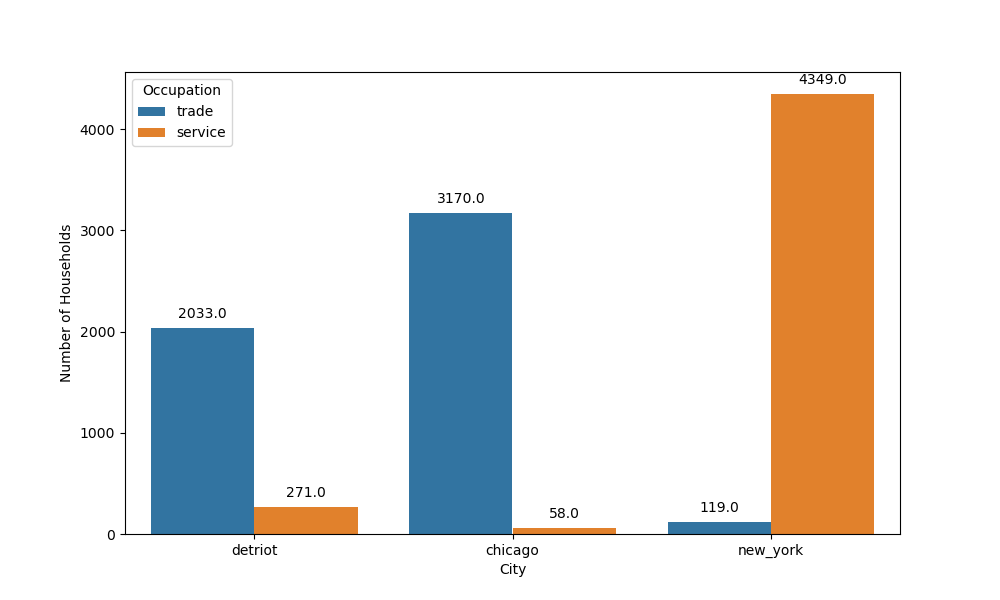
\includegraphics[width=\textwidth]{../simulations/graphs/city_pop.png}
            \caption{Initial Distribution of Populations}
            \label{city_pop}
        \end{minipage}%
        \begin{minipage}{0.5\textwidth}
            \centering
            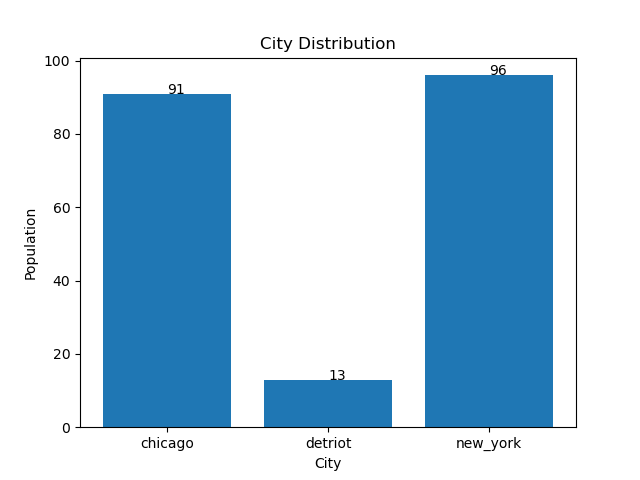
\includegraphics[width=\textwidth]{../simulations/graphs/c_shock.png}
            \caption{Post Detriot Shock}
            \label{c_shock}
        \end{minipage}
    \end{figure}
\end{frame}

\section{To Do List}

\begin{frame}
    \frametitle{Table of Contents}
    \setbeamertemplate{section in toc}[sections numbered]
    \tableofcontents[currentsection]
\end{frame}

\begin{frame}
    \centering
    \frametitle{To Do List}
    \begin{itemize}
        \setlength{\itemsep}{3em}
        \item Estimation equation for parameters.
        \item Obtain wage and emplyment for American cities.
        \item Run counterfacutals.
              \begin{itemize}
                  \item China shock.
              \end{itemize}
    \end{itemize}
\end{frame}

\end{document}